% VUT FIT MITAI
% MSZ 2021/2022
% Author: Vladimir Dusek
% Login: xdusek27

%%%%%%%%%%%%%%%%%%%%%%%%%%%%%%%%%%%%%%%%%%%%%%%%%%%%%%%%%%%%%%%%%%%%%%%%%%%%%%%%

% Path to figures
\graphicspath{{pds/rizeni_toku_a_prevence_zahlceni}}

%%%%%%%%%%%%%%%%%%%%%%%%%%%%%%%%%%%%%%%%%%%%%%%%%%%%%%%%%%%%%%%%%%%%%%%%%%%%%%%%

\chapter{Řízení toku dat (flow-control) a prevence zahlcení (congestion-control) na transportní vrstvě (MP-TCP, QUIC, SCTP, DCCP).}

%%%%%%%%%%%%%%%%%%%%%%%%%%%%%%%%%%%%%%%%%%%%%%%%%%%%%%%%%%%%%%%%%%%%%%%%%%%%%%%%

\section{Metadata}

\begin{compactitem}
    \item Předmět: Přenos dat, počítačové sítě a protokoly (PDS)
    \item Přednáška:
    \begin{compactitem}
        \item \path{02-transportni-protokoly.pdf}
    \end{compactitem}
    \item Záznam:
    \begin{compactitem}
        \item 2021-02-19
    \end{compactitem}
\end{compactitem}

%%%%%%%%%%%%%%%%%%%%%%%%%%%%%%%%%%%%%%%%%%%%%%%%%%%%%%%%%%%%%%%%%%%%%%%%%%%%%%%%

\section{Úvod a kontext}

% src: https://linuxhint.com/network-osi-layers-explained
\begin{figure}[H]
    \centering
    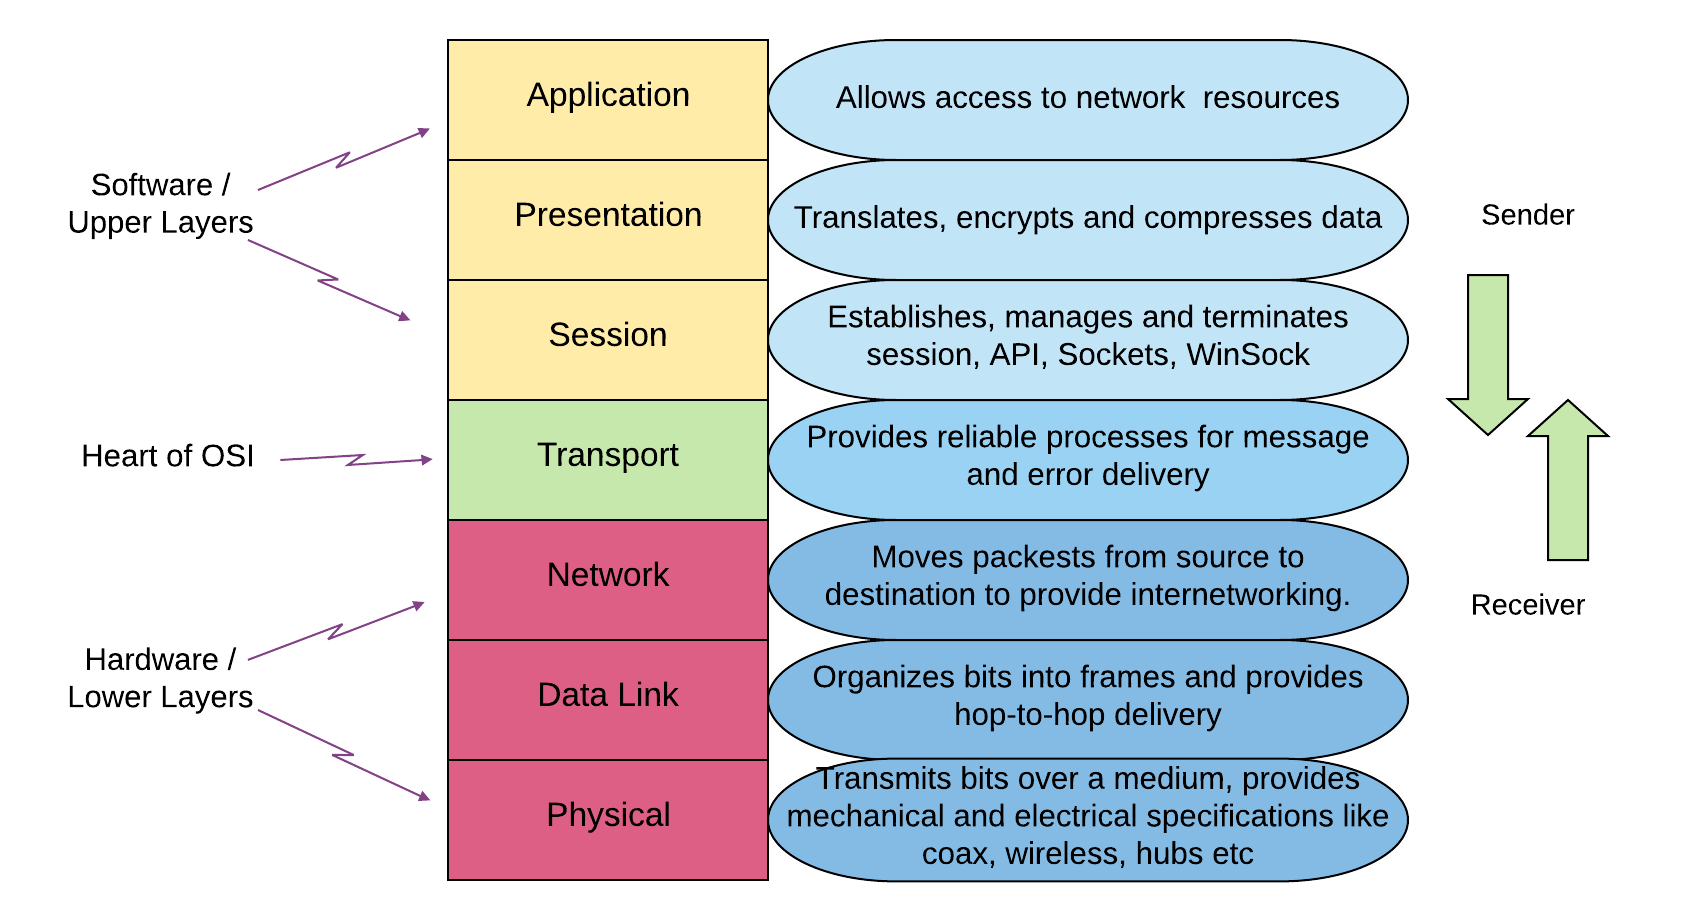
\includegraphics[width=1\linewidth]{osi_model_linuxhint.png}
    \caption{Příklad OSI modelu z Linuxhint.}
\end{figure}

% src: https://cs.wikipedia.org/wiki/Soubor:OSI_Model_v1.svg
\begin{figure}[H]
    \centering
    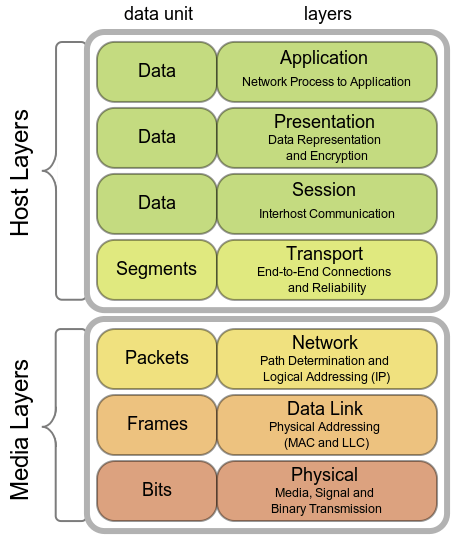
\includegraphics[width=0.65\linewidth]{osi_model_wiki.png}
    \caption{Příklad OSI modelu z Wiki.}
\end{figure}

% Které problémy řeší transportní vrstva? Ztráta packatu, zahlcení, multiplexing
\paragraph*{Transportní vrstva} Transportní vrstva je název čtvrté vrstvy modelu vrstvové síťové architektury (ISO/OSI model). Leží mezi vrstvou síťovou (L3) a aplikační (L7). \begin{compactitem}
    \item Činnost na straně odesílatele: obdrží data z aplikační vrstvy, nasegmentuje je a ke každému segmentu/datagramu přidá L4 hlavičku.
    \item Činnost na straně příjemce: obdrží segmenty/datagramy, které uspořádá do správného pořadí (\textit{out-of-order} doručení), předá je aplikační vrstvě.
    \item Rozhraní mezi L4 a L7: sockety.
    \item Zodpovědnost za \textit{end-to-end} spojení.
    \item Adresuje aplikace (pomocí portových čísel).
    \item \textit{Quality of Service} -- zotavení se z chyb, spolehlivost, řízení toku, řízení zahlcení.
\end{compactitem}

\paragraph*{TCP (\textit{Transmission Control Protocol})} \begin{compactitem}
    \item Spolehlivé doručení
    \item Řízení toku a zahlcení
    \item Doručování v pořadí
    \item Duplexní
    \item 3 fáze spojení -- navázení, přenos dat, ukončení
\end{compactitem}

\paragraph*{UDP (\textit{User Datagram Protocol})} \begin{compactitem}
    \item Nespolehlivé doručení (\textit{best effort})
    \item Má minimální režii
    \item Duplexní
\end{compactitem}

\paragraph*{bandwith, throughput, goodput} \begin{compactitem}
    \item Bandwith -- šířka pásma, maximální přenos dat danou cestou v jeden moment
    \item Throughput -- propustnost komunikace na úrovni protokolu
    \item Goodput -- propustnost komunikace na úrovni aplikace (throughput $-$ režie)
\end{compactitem}

\paragraph*{data, segment, datagram, paket, rámec, bit} \begin{compactitem}
    \item Data -- aplikační vrstva (L7)
    \item Segment -- transportní vrstva (L4), TCP
    \item Datagram -- transportní vrstva (L4), UDP
    \item Paket -- síťová vrstva (L3)
    \item Rámec -- linková vrstva (L2)
    \item Bit -- fyzická vrstva (L1)
\end{compactitem}

\paragraph*{Bitové chyby} \begin{compactitem}
    \item \uv{Přeskočení bitu} (\textit{bit swapping}), jde o chyby na úrovni zpracování informace uzlem v síti (typicky spojené s přenosovým médiem)
    \item Zabýváme se jimi na úrovni L2
    \item Řešením je obvykle redundance (Hammingův kód, CRC, Viterbiho algoritmus, \dots)
\end{compactitem}

\begin{figure}[H]
    \centering
    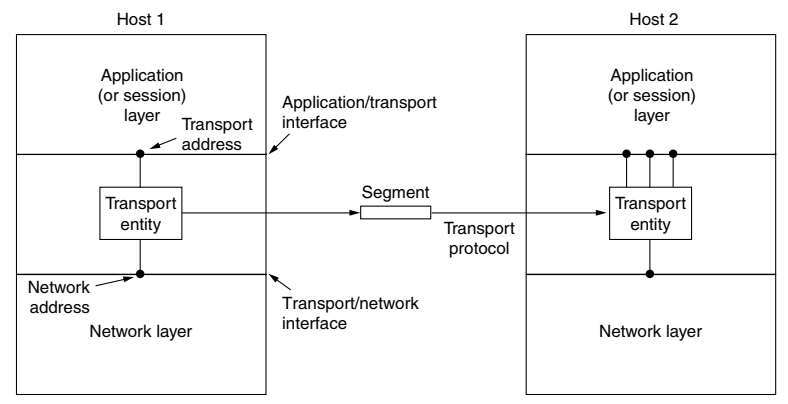
\includegraphics[width=1\linewidth]{l4.png}
    \caption{Transportní vrstva (L4).}
\end{figure}

%%%%%%%%%%%%%%%%%%%%%%%%%%%%%%%%%%%%%%%%%%%%%%%%%%%%%%%%%%%%%%%%%%%%%%%%%%%%%%%%

\section{Paketové chyby}

\begin{compactitem}
    \item Jde o chyby na úrovni přenosu informace mezi dvěma uzly
    \item Zabýváme se jimi na úrovni L4
    \item Řešením je obvykle znovuzaslání
    \item Můžeme měřit: \begin{compactitem}
        \item PER (\textit{packet error rate}) $$PER = \frac{\text{pocet chybnych paketu}}{\text{pocet prenesenych paketu}}$$
        \item BER (\textit{bit error rate}) $$BER = \frac{\text{pocet chybnych bitu}}{\text{pocet prenesenych bitu}}$$
    \end{compactitem}
\end{compactitem}

\subsection*{Druhy paketových chyb}

\paragraph*{Ztráta (zpoždění) paketu} Jak může dojít ke ztrátě (zpoždění) paketu? \begin{compactitem}
    \item Neopravitelná bitová chyba (rámec je zahozen na L2)
    \item Zahlcení linky (routery jsou přetíženy)
    \item Špatné směrovací tabulky (paket jde špatnou cestou, nebo cyklí a vyprší mu TTL)
\end{compactitem}

\paragraph*{Ztráta fragmentovaných dat} Nějaký router po cestě směruje paket na rozhraní, které má menší MTU (\textit{Maximum Transmission Unit} -- označení pro maximální velikosti paketu), to znamená, že paket musí rozdělit na více menších paketů (fragmentů). Fragment se pak může ztratit ze stejného důvodu jako standardní nefragmentovaný paket.

\paragraph*{Duplicita paketu} Příjemce obdržuje stále paket se stejným sekvenčním číslem. Odesílatel si myslí, že se paket k příjemci nikdy nedostal. Proč? \begin{compactitem}
    \item Ztratí se potvrzení o přijetí paketu.
\end{compactitem}

\paragraph*{Vložení paketu} Příjemce obdrží paket, který do spojení nepatří. Jak k tomu může dojít? \begin{compactitem}
    \item Přijetí zpožděného paketu, který dorazil až po skončení jednoho a začátku dalšího separátního datového toku.
    \item Podvrhávání paketu útočníkem snažícím se narušit integritu sítě.
    \item Paket je chybou \uv{zvláštně zmrzačen}, tak, že chybu nelze rozpoznat (např. je změněm bit v cílové IP adrese), a je směrován jinému příjemci.
\end{compactitem}

\paragraph*{Změna pořadí} Vychází z designu počítačových sítí, kdy paketu mohou proudit různými cestami a s různým zpožděním. Data jsou \textit{out-of-order} a příjemce je musí přeuspořádat.

\subsection*{Detekce paketové chyby}

Paketové chyby detekujeme pomocí sekvenčních čísel. Sekvenční číslo je jedinečné číslo paketu, které identifikuje jeho pořadí v rámci datového toku. Tímto poznáme ztrátu, duplicitu i změnu pořadí. Jak rozpoznat ztrátu od zpoždění?

\paragraph*{Timeout} Může být fixní, ale v lepším případě odvozen od RTT (\textit{round trip time} -- \uv{cesta tam a zpátky})).

\paragraph*{Negativní potvrzování} Paket jsem dostal (ACK) / paket jsem nedostal (NACK). Pokud je příčina zpoždění zahlcení, tak tento přístup linku ještě více zahltí.

\subsection*{Korekce paketových chyb}

Pokud paket nedorazil, odesílatel ho pošle znovu. Tzv. \textit{Automatic Repeat/Request} (ARQ) -- Čeká se na ACK, když nepřijde do timeoutu, dojde k znovuzaslání. Princip tzv. klouzavého okna (\textit{sliding windows}). Existují 3 strategie.

\paragraph*{Stop and wait} \begin{compactitem}
    \item Klouzavé okno o velikosti 1.
    \item Odesílatel pošle paket a čeká na potvrzení, pak pošle další.
    \item Špatná efektivita využití pásma.
\end{compactitem}

\paragraph*{Go back n} \begin{compactitem}
    \item Buffer na straně odesílatele.
    \item Příjemce potvrzuje naposledy přijatým paketem (např. pošle ACK2 znamená, že dostal pakety 0, 1, 2).
    \item Plýtvání při znovuzaslání (např. odesílatel pošle 5 paketů, ztratí se první, musí poslat znovu všech 5).
\end{compactitem}

\paragraph*{Selective repeat} \begin{compactitem}
    \item Buffery jsou na obou stranách.
    \item Efektivní využítí šířky pásma, ale složitější implementace.
    \item Příjemce potvrzuje: \begin{compactitem}
        \item Naposledy přijatým paketem
        \item Bitovou maskou (co přijal a co ne)
        \item NACK (co chce zaslat znovu)
    \end{compactitem}
\end{compactitem}

%%%%%%%%%%%%%%%%%%%%%%%%%%%%%%%%%%%%%%%%%%%%%%%%%%%%%%%%%%%%%%%%%%%%%%%%%%%%%%%%

\section{Řízení toku dat}

%%%%%%%%%%%%%%%%%%%%%%%%%%%%%%%%%%%%%%%%%%%%%%%%%%%%%%%%%%%%%%%%%%%%%%%%%%%%%%%%

\section{Prevence zahlcení}

\todo{todo}

%%%%%%%%%%%%%%%%%%%%%%%%%%%%%%%%%%%%%%%%%%%%%%%%%%%%%%%%%%%%%%%%%%%%%%%%%%%%%%%%

\section{MP-TCP}

\todo{todo}

%%%%%%%%%%%%%%%%%%%%%%%%%%%%%%%%%%%%%%%%%%%%%%%%%%%%%%%%%%%%%%%%%%%%%%%%%%%%%%%%

\section{QUIC}

\todo{todo}

%%%%%%%%%%%%%%%%%%%%%%%%%%%%%%%%%%%%%%%%%%%%%%%%%%%%%%%%%%%%%%%%%%%%%%%%%%%%%%%%

\section{SCTP}

\todo{todo}

%%%%%%%%%%%%%%%%%%%%%%%%%%%%%%%%%%%%%%%%%%%%%%%%%%%%%%%%%%%%%%%%%%%%%%%%%%%%%%%%

\section{DCCP}

\todo{todo}
